\section*{Теоретическая часть:}
\begin{enumerate}
    \item Получение эллиптически поляризованного света. \\
    \begin{figure}[h!]
        \noindent\centering{
            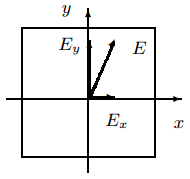
\includegraphics[height = 4cm]{Selection_048.png}
        }
        \caption{Разложение линейно поляризованного света по главным направлениям двоякопреломляющей пластинки.}
    \end{figure} \\
    
    
    \begin{figure}[h!]
        \noindent\centering{
            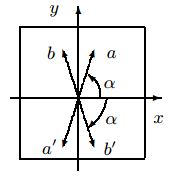
\includegraphics[height = 4cm]{Selection_049.png}
        }
        \caption{Поворот направления колебаний с помощью пластинки в $\lambda / 2$.}
    \end{figure} 
    \newpage
    \item Пластинка чувствительного оттенка. \\
    \begin{figure}[h!]
        \noindent\centering{
            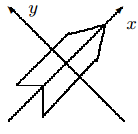
\includegraphics[height = 4cm]{Selection_050.png}
        }
        \caption{}
    \end{figure} \\
    
    \item Интерференция поляризованных лучей.
    \begin{figure}[h!]
        \noindent\centering{
            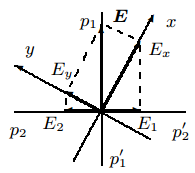
\includegraphics[height = 4cm]{Selection_051.png}
        }
        \caption{К объяснению интерференции поляризованных лучей.}
    \end{figure} \\
    
\end{enumerate}